\documentclass[tikz,border=2mm]{standalone}

\usepackage{bm}
\usepackage{xcolor}
\usetikzlibrary{arrows,positioning}
\usetikzlibrary{arrows.meta}

\begin{document}

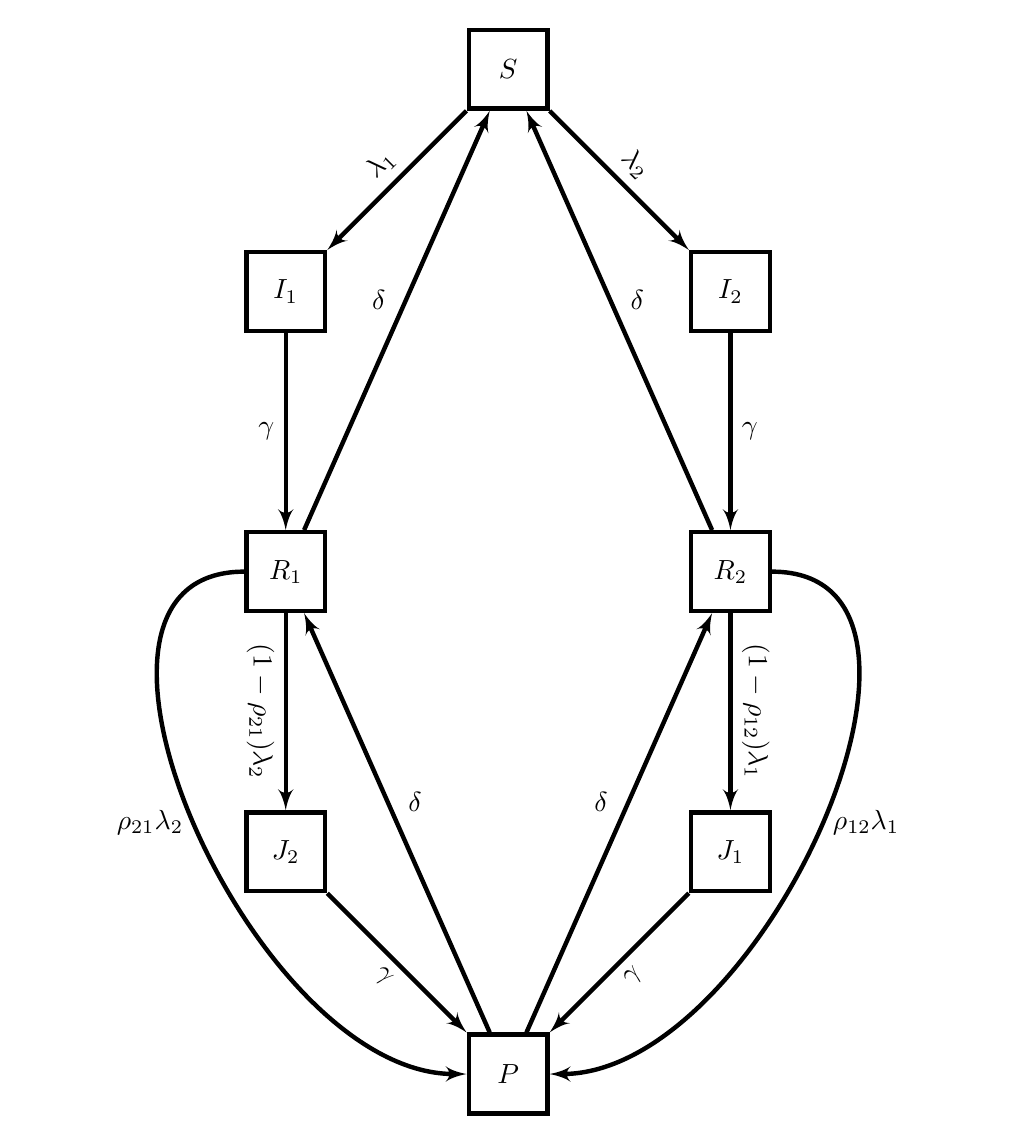
\begin{tikzpicture}[node distance=2.5cm,auto,>=latex',every node/.append style={align=center},int/.style={draw, minimum size=1cm},inverter/.style={rectangle,draw,inner sep=2pt,minimum size=6mm},posnode/.style={shape=rectangle, draw=orange, line width=2},
  negnode/.style={shape=rectangle, draw=black, line width=2}]
    \node [int, ultra thick] (S)             {$S$};
    \node [int, below left=of S, ultra thick] (I1)             {$I_1$};
    \node [int, below=of I1, ultra thick] (R1)             {$R_1$};
    \node [int, below right=of S, ultra thick] (I2)             {$I_2$};
    \node [int, below=of I2, ultra thick] (R2)             {$R_2$};
    \node [int, below=of R1, ultra thick] (J2)             {$J_2$};
    \node [int, below=of R2, ultra thick] (J1)             {$J_1$};
    \node [int, below left=of J1, ultra thick] (R)             {$P$};
    \path[->, ultra thick, above, sloped] (S) edge node {$\lambda_1$} (I1);
    \path[->, ultra thick, above, sloped] (S) edge node {$\lambda_2$} (I2);
    \path[->, ultra thick, left] (I1) edge node {$\gamma$} (R1);
    \path[->, ultra thick, right] (I2) edge node {$\gamma$} (R2);
    \path[->, ultra thick, below, sloped] (R1) edge node {$(1-\rho_{21})\lambda_2$} (J2);
    \path[->, ultra thick, above, sloped] (R2) edge node {$(1-\rho_{12})\lambda_1$} (J1);
    \path[->, ultra thick, below, sloped] (J2) edge node {$\gamma$} (R);
    \path[->, ultra thick, below, sloped] (J1) edge node {$\gamma$} (R);
    \path[->, ultra thick, above right] (R) edge node {$\delta$} (R1);
    \path[->, ultra thick, above left] (R) edge node {$\delta$} (R2);
    \path[->, ultra thick, above left] (R1) edge node {$\delta$} (S);
    \path[->, ultra thick, above right] (R2) edge node {$\delta$} (S);
    \path[->, ultra thick, right, out=0, in=0] (R2.east) edge node {$\rho_{12}\lambda_1$} (R.east);
    \path[->, ultra thick, left, out=180, in=180] (R1.west) edge node {$\rho_{21}\lambda_2$} (R.west);
\end{tikzpicture}
\end{document}
